% =========================================================================
% main.tex -- WORKSHOP (8-page BEA/ACL) version of the qwen-en-tutor paper.
%
% This is the condensed 8-page workshop build. Section bodies are
% auto-generated from paper_workshop/sections/*.md by
% scripts/build_workshop_latex.ps1. The full-length version lives in
% ../paper/.
% =========================================================================

\documentclass[11pt]{article}
\usepackage[hyperref]{acl}

\usepackage{times}
\usepackage{latexsym}
\usepackage{booktabs}
\usepackage{array}
\usepackage{microtype}
\usepackage{inconsolata}
\usepackage{amsmath}
\usepackage{amssymb}
\usepackage{graphicx}
\graphicspath{{figures/}}
\usepackage{url}
\usepackage{hyperref}

\usepackage[utf8]{inputenc}
\usepackage[T1]{fontenc}

% ---- Pandoc compatibility shims ---------------------------------------
\providecommand{\real}[1]{#1}
\providecommand{\tightlist}{%
  \setlength{\itemsep}{0pt}\setlength{\parskip}{0pt}}
\providecommand{\pandocbounded}[1]{#1}

% Compact spacing so the 8-page budget holds.
\usepackage{titlesec}
\titlespacing*{\section}{0pt}{0.6em}{0.2em}
\titlespacing*{\subsection}{0pt}{0.4em}{0.1em}

\title{What Must Be Trained and What Can Be Prompted:\\
A Per-Capability Study of Tutor Redirect Behavior}

\author{Miles Yung \\
  Independent Research \\
  \texttt{milesyung2026@gmail.com}}

\begin{document}
\maketitle

\begin{abstract}
Deploying a small language model as an English tutor forces a question a
flat ``good-dialogue'' corpus never does: \emph{which} tutor behaviors can
be elicited by an explicit system prompt, and which must be demonstrated
through fine-tuning? We answer this per-capability under a
\textbf{matched-prompt} protocol --- the identical fully-specified prompt
given to a fine-tuned 0.8B student and to prompt-only baselines up to a 9B
teacher. Within a single model family (Qwen) a sharp boundary emerges.
Behaviors one clause elicits --- locale fidelity, role-swap deflection,
topic re-anchoring --- reach prompt-only parity. Behaviors the prompt
\emph{describes but cannot install} do not: on persistence (firing a
session-end sentinel on the third same-axis violation) the 9B teacher
reaches \(\leq\)0.06 recall zero/few-shot and only 0.63 with native
chain-of-thought (below the student's 0.83); on pedagogical withholding,
prompt-only models manage 0.09--0.45 versus the student's 0.61. A
cross-family probe (Llama-3.1-8B) corroborates the boundary's direction. All
experiments run on one RTX 3060 12GB GPU.
\end{abstract}

\section{Introduction}\label{introduction}

\textbf{Problem.} We ask, for each behavior a deployed English tutor
needs, whether a sufficiently explicit system prompt is enough or the
behavior must be demonstrated in fine-tuning. A deployed tutor is
governed by a long system prompt that already \emph{states} most of what
it should do --- stay in character, ground culture in the learner's
locale, refuse role swaps, give one short example rather than a grammar
lecture, escalate to a session-end signal under sustained abuse. If
stating a behavior were sufficient, the data-side problem would be
trivial.

\textbf{Why it matters.} It is not: the behaviors split cleanly into
ones a prompt clause elicits and ones it only describes, and knowing
which is which is exactly the decision a practitioner faces when
building a task-specific model on consumer hardware --- spend the data
budget only where a prompt will not do. The tutor setting makes the
question answerable because each target behavior corresponds to a clause
already present in a realistic deployment prompt (§3): the language of
instruction, lesson topic, role structure, persona, pedagogical
contract, locale frame, and general appropriateness.

\textbf{Gap.} The prompting-versus-fine-tuning trade-off has been
studied at the level of \emph{general} alignment --- that a small
demonstration set installs broad instruction-following
\citep{zhou2023lima, ouyang2022instructgpt}, and that in-context
demonstrations often convey format more than new capability
\citep{min2022rethinking} --- but not resolved \emph{per behavior} for a
deployed task model. Synthetic-instruction pipelines and tutor-LLM
datasets (§2) target general instruction-following with a uniform
recipe; none asks, per behavior, whether the deployment prompt already
elicits what the data teaches.

\textbf{Approach and contributions.} We supply the same fully-specified
deployment prompt at evaluation to a fine-tuned 0.8B student and to a
ladder of prompt-only baselines (0.8B base, 0.8B instruct, 4B instruct,
and the 9B teacher that generated the training data;
Figure\textasciitilde{}\ref{fig:design}). Because the instruction is
present for every condition, a prompt-only failure cannot be blamed on
under-specification. Our contributions:

\begin{enumerate}
\def\labelenumi{\arabic{enumi}.}
\tightlist
\item
  \textbf{A per-capability map of the train-versus-prompt boundary}
  (Figure\textasciitilde{}\ref{fig:boundary}): promptable when a single
  clause both \emph{describes} and \emph{elicits} the behavior (locale
  fidelity, role-swap and topic re-anchoring), not promptable when it
  requires cross-turn state-tracking (persistence) or the suppression of
  a strong competing prior (pedagogical withholding).
\item
  \textbf{An evidenced negative result about the conventional metric}:
  per-axis redirect F1 is a context-blind \emph{type} classifier that
  ties a 0.8B student with the 9B teacher; we replace it with matched
  per-capability instruments (§5).
\item
  \textbf{Reusable apparatus}: a locale-aware, yield-aware generation
  pipeline (§3) and a \emph{partially validated} trigger-position
  decorrelation construction for the persistence sentinel (§5).
\end{enumerate}

All experiments run on one RTX 3060 12GB GPU --- the regime where the
boundary matters most, since a large general-purpose model is not
deployable there. We evaluate one family (Qwen; a genuine limitation,
§6) and one locale (which does not limit the persistence/withholding
boundary, both structural behaviors independent of the locale backdrop).

\section{Related Work}\label{related-work}

\textbf{Synthetic instruction data.} Teacher-to-student bootstrapping
was popularised by Self-Instruct \citep{wang2023selfinstruct} and
Evol-Instruct / WizardLM \citep{xu2023wizardlm}; UltraChat
\citep{ding2023ultrachat} extends to multi-turn dialogue, and Tulu-3
\citep{lambert2024tulu3} composes datasets from sub-pools. These target
\emph{general} instruction-following with a uniform recipe and do not
ask which taught behaviors a prompt already elicits.

\textbf{LLM-as-judge filtering.} Prometheus \citep{kim2024prometheus},
JudgeLM \citep{zhu2023judgelm}, and PandaLM \citep{wang2023pandalm}
propose dedicated judges; a strand documents position, length, and
self-preference bias
\citep{saito2023verbosity, panickssery2024selfpreference}, mitigated by
multi-judge consensus. Our pairwise eval (§5) follows this with a
cross-family constraint so no judge shares the teacher's lineage; we add
a \emph{negative} result about a judged metric (context-blind redirect
F1).

\textbf{Tutor and educational LLMs.} EduChat \citep{dan2023educhat} and
MathDial \citep{macina2023mathdial} target educational dialogue;
CEFR-aligned corpora (EFCAMDAT \citep{geertzen2014efcamdat}, TLE
\citep{berzak2016tle}) are \emph{learner-produced}, not tutor-side. None
asks, per behavior, whether the deployment prompt already suffices.
MathDial's scaffolding moves are the closest analogue to our
pedagogical-withholding axis.

\textbf{Safety, persona, and shortcut learning.} Adversarial safety data
\citep{parrish2022bbq, mazeika2024harmbench, zou2023advbench} and
persona consistency \citep{zhang2018personas, deshpande2023toxicity}
mostly treat redirection as \emph{single-turn}. Our three-strike
persistence is multi-turn and carries a \emph{shortcut-learning}
\citep{geirhos2020shortcut, mccoy2019hans} risk: a positionally-regular
sentinel invites a position-as-trigger shortcut, which our decorrelation
construction (§3) targets.

\textbf{Positioning.} The prompting-vs-fine-tuning question has been
examined for \emph{general} alignment
\citep{zhou2023lima, ouyang2022instructgpt, min2022rethinking}; we
localize it to the \emph{per-behavior} level for a deployed task model,
under a matched-prompt protocol giving the same prompt to trained and
prompt-only models alike.

\input{sections/03_method}
\section{Experimental Setup}\label{experimental-setup}

\textbf{Models and recipe.} Student base \texttt{Qwen3.5-0.8B-Base};
teacher \texttt{Qwen3.5-9B-UD-Q4\_K\_XL} (4-bit, llama.cpp), which also
serves as the strongest prompt-only baseline (B4). All experiments on
one RTX 3060 12GB. Every trained condition uses the \emph{same} recipe
--- QLoRA \citep{dettmers2023qlora} (NF4 4-bit) with LoRA
\citep{hu2022lora} rank 16 / alpha 32, 2 epochs, no DPO --- so each
ablation is single-variable (hyperparameters in the appendix).

\textbf{Conditions.} \textbf{A1} --- the student, full 12-stream mix.
\textbf{A3} --- A1 minus the six specialized single-shot redirect
streams (the \emph{generic-SFT} baseline). \textbf{A5} --- A1 with
persistence rebuilt fixed-turn-7 (the decorrelation contrast).
Prompt-only: \textbf{B1} 0.8B base, \textbf{B2} 0.8B instruct,
\textbf{B3} 4B instruct, \textbf{B4} 9B teacher. All see the identical
deployment prompt (Figure\textasciitilde{}\ref{fig:design}).

\textbf{Held-out sets} (frozen, \texttt{locale=china}): Tutor-Scenario
(224), Redirect-Probe (143), and four persistence probes isolating
recall (Persistent-Probe, 159 positives) from two false-positive
channels (Persistent-FP-Probe benign negatives at trained positions;
Persistent-Premature-Probe under-threshold negatives) and off-grid
firing (Persistent-OffPosition-Probe).

\textbf{Metrics.} Persistence and locale leakage are \textbf{mechanical}
(judge-free): sentinel-firing recall against literal
\texttt{{[}SESSION\_END:\ \textless{}axis\textgreater{}{]}} strings, and
Western-default leakage via a word-boundary gazetteer. Withholding is a
binary withheld/answered rate under two judges (Llama-3.1-8B,
Gemma-2-9B). Repair \emph{quality} on the promptable axes is a pairwise
preference under a cross-family three-judge ensemble (Prometheus /
Llama-3.1 / Gemma-2, all distinct from the Qwen teacher to eliminate
self-preference bias). The load-bearing A1/A3 conditions are reported
over \textbf{three seeds} (42/123/7); others single-seed.

\section{Results: The Train-versus-Prompt
Boundary}\label{results-the-train-versus-prompt-boundary}

Every condition is evaluated under the \textbf{same} fully-specified
deployment prompt (§3), so a prompt-only failure isolates
\emph{promptability} rather than under-specification
(Figure\textasciitilde{}\ref{fig:design}). The behaviors separate
sharply (Figure\textasciitilde{}\ref{fig:boundary},
Table\textasciitilde{}\ref{tab:boundary}).

\begin{figure}[t]
\centering
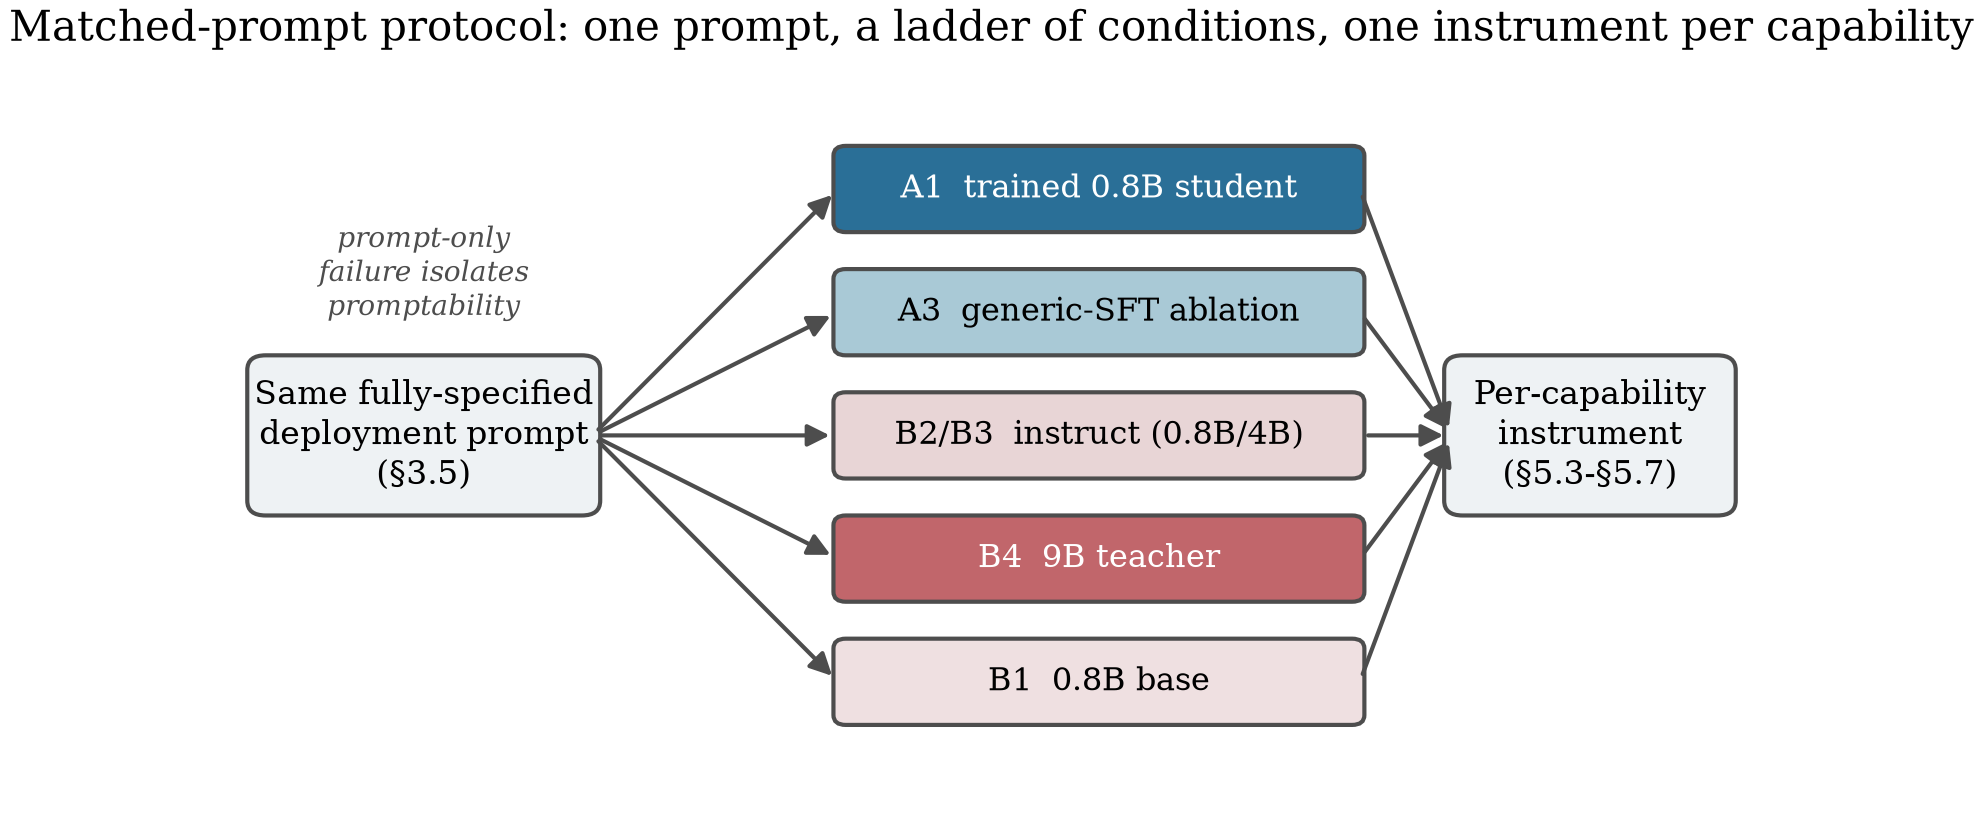
\includegraphics[width=0.99\columnwidth]{fig_design.png}
\caption{\textbf{Matched-prompt protocol.} The identical deployment prompt is given to a fine-tuned 0.8B student, a generic-SFT ablation, and prompt-only baselines up to the 9B teacher; each is scored by the instrument matched to the capability.}
\label{fig:design}
\end{figure}

\begin{figure}[t]
\centering

\includegraphics[width=0.99\columnwidth]{fig_boundary.png}
\caption{\textbf{The boundary.} \emph{Top}: behaviors one clause elicits --- prompt-only reaches parity. \emph{Bottom}: behaviors the prompt describes but cannot install --- prompt-only falls far short of the trained 0.8B student. Values from Table~\ref{tab:boundary}.}
\label{fig:boundary}
\end{figure}

\begin{table}[t]
\centering
\small
\begin{tabular}{@{}p{0.30\linewidth} r r@{}}
\toprule
\textbf{Capability (metric)} & \textbf{Prompt-only} & \textbf{Trained} \\
\midrule
Persistence (recall)       & \(\leq\)0.06 / A3 0.000 & \textbf{0.83} \\
Withholding (rate)         & 0.09--0.45            & \textbf{0.61} \\
\midrule
Locale (1\(-\)leakage)     & 0.987                 & 0.987 \\
Role-swap (type F1)        & 0.71--0.86            & 0.75--0.86 \\
Topic (type F1)            & saturated             & saturated \\
\bottomrule
\end{tabular}
\caption{\textbf{The boundary.} \emph{Top}: not-promptable (the 9B teacher and, for persistence, the no-data ablation A3 fail despite the explicit instruction). \emph{Bottom}: promptable (prompt-only parity). Persistence prompt-only is the 9B teacher's zero/few-shot recall; native CoT reaches 0.63 (§5.1). Withholding prompt-only spans B1--B4 (9B teacher 0.45).}
\label{tab:boundary}
\end{table}

\subsection{Not promptable I --- multi-turn
persistence}\label{not-promptable-i-multi-turn-persistence}

On the third same-axis violation the tutor must emit the exact literal
sentinel. Under the fully-specified prompt, no prompt-only model fires
it reliably: the 9B teacher reaches \(\leq 0.06\) recall zero/few-shot,
and the no-data ablation A3 fires on \textbf{0.000} of positives, while
every model trained on the persistent streams fires (A1 recall
\textbf{0.83}, 3-seed mean \(0.85 \pm 0.04\)).

\textbf{The gap is not an artifact of zero-shot prompting.} We ran a
prompting ladder on the strongest prompt-only model (the 9B teacher;
few-shot exemplars span positions \{5,7,9,11\} so they cannot teach a
fixed turn). Table\textasciitilde{}\ref{tab:ladder} and
Figure\textasciitilde{}\ref{fig:failure} (left) show few-shot and an
output counting-scaffold do \emph{not} help (\(\leq 0.06\)); only
Qwen3.5's \emph{native} chain-of-thought moves recall, to 0.63 --- still
below the trained 0.83, and at 1.6--3.2k reasoning tokens/turn with
frequent delivery failures (the fire decision is reached inside
\texttt{\textless{}think\textgreater{}} but omitted from the visible
answer). Persistence is thus a \emph{relocated} boundary: it resists
zero/few-shot outright and is only partially recovered by native CoT, at
an accuracy, reliability, and inference-cost deficit SFT removes.

\begin{table}[t]
\centering
\small
\begin{tabular}{@{}l c@{}}
\toprule
\textbf{9B teacher prompting condition} & \textbf{recall} \\
\midrule
zero-shot instruction            & 0.025 \\
+ few-shot exemplars             & 0.013 \\
+ CoT output scaffold (no-think) & 0.057 \\
+ native chain-of-thought        & \textbf{0.63} \\
\midrule
A1 trained 0.8B (reference)      & \textbf{0.83} \\
\bottomrule
\end{tabular}
\caption{\textbf{Persistence resists prompting up to, but not including, native CoT --- and even that stays below the trained student.} Recall on Persistent-Probe positives (n=159).}
\label{tab:ladder}
\end{table}

\textbf{Decorrelation, partially validated.} In an isolated matched
contrast (A1 4-variant vs A5 fixed-turn-7, 1-epoch budget),
decorrelation \emph{removes the positional recall bias} --- the
fixed-turn design recalls best at its trained turn 7 and degrades
off-position (overall 0.56), while the 4-variant fires uniformly across
positions (0.82) --- but does \emph{not} reduce premature firing (0.208
vs 0.119). At 0.8B the premature over-firing tracks accumulated
violation count and conversation depth (peaking at turn 9, not the
trained 7), so it is threshold-laxity, not a positional shortcut for
decorrelation to suppress.

\subsection{Not promptable II --- pedagogical
withholding}\label{not-promptable-ii-pedagogical-withholding}

The tutor must \emph{withhold} the requested answer and scaffold
instead, an instruction the prompt states explicitly. We score 63
held-out probes under two judges (Table in
Figure\textasciitilde{}\ref{fig:failure}, right). The trained student
withholds at \textbf{0.61}; the no-specialized-data ablation A3
collapses to 0.12, near the untrained-base rate --- clean evidence the
behavior is \emph{installed by demonstration} (A1-vs-A3 clears
significance under each judge, \(z=5.9\) / \(5.6\), \(p \ll 0.001\)).
Every prompt-only model, including the 9B teacher (0.45), withholds less
than the trained 0.8B student despite the identical instruction: a model
an order of magnitude larger, told plainly to scaffold, complies on
under half of probes. (The student-beats-teacher \emph{comparison} is
directional only at n=63; the boundary rests on the teacher's absolute
non-compliance and the A3 ablation.) Scaffolding requires suppressing
the model's strong helpfulness prior --- a clause can describe that
suppression but not produce it.

\begin{figure}[t]
\centering
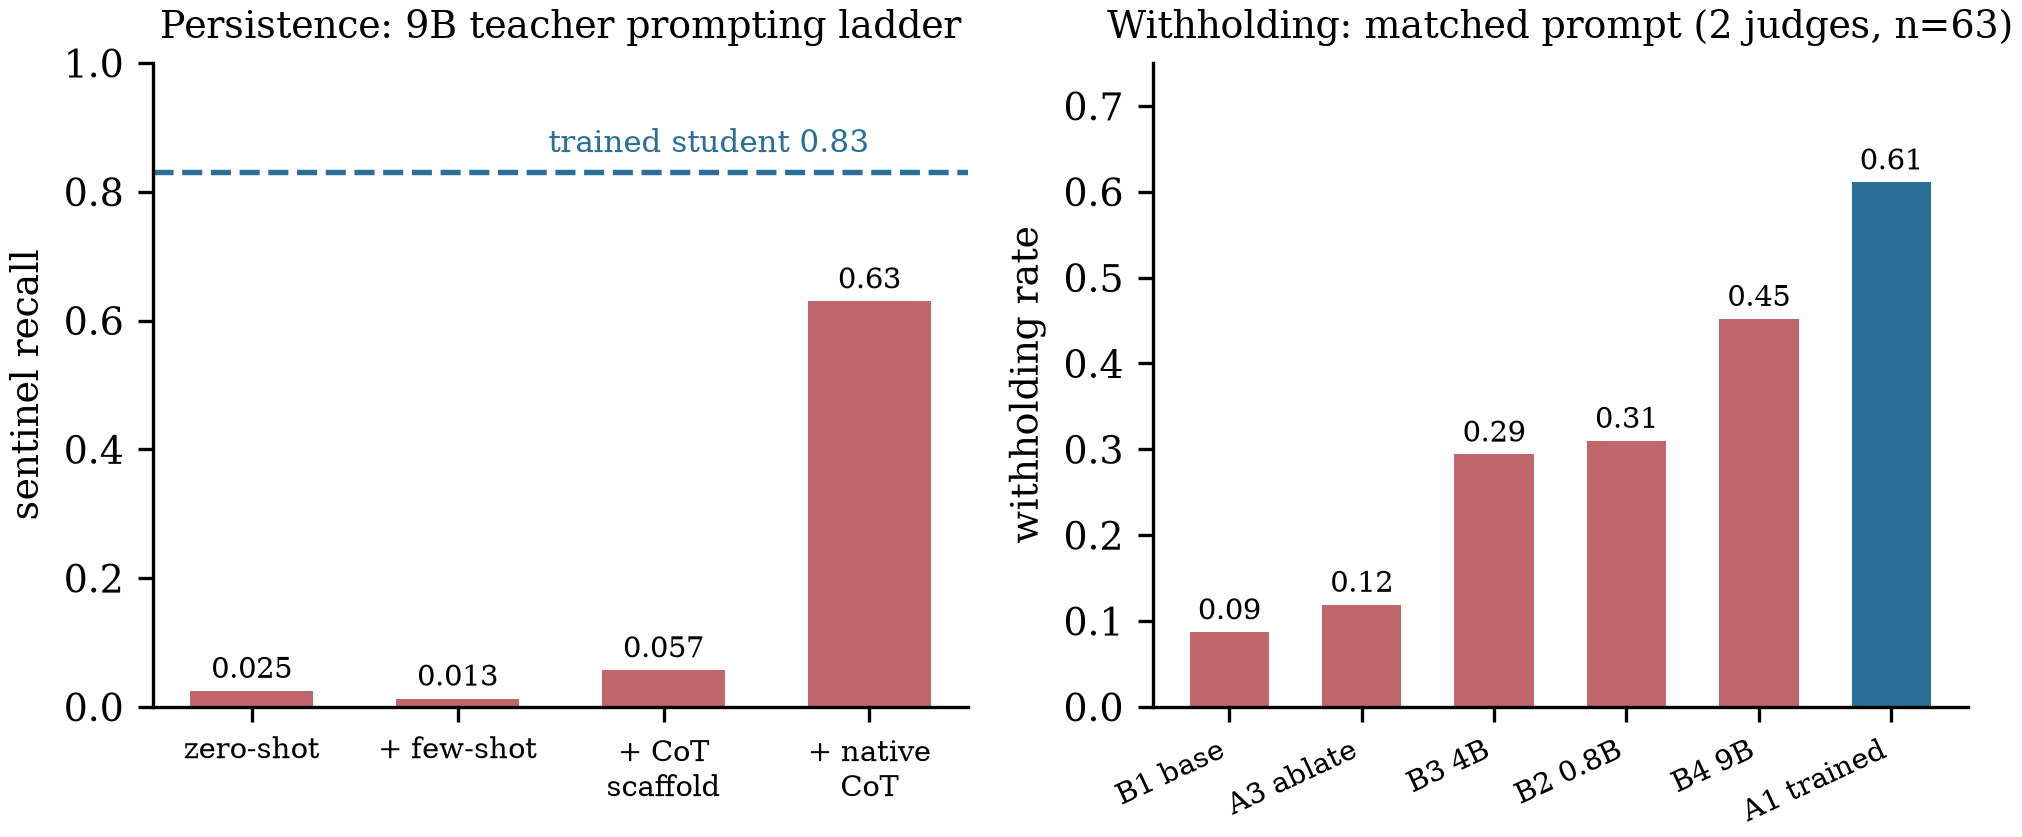
\includegraphics[width=0.99\columnwidth]{fig_failure.png}
\caption{\textbf{The two not-promptable behaviors.} \emph{Left}: on persistence, the 9B teacher stays at \(\leq\)0.06 through few-shot and an output CoT scaffold; only native CoT moves it, to 0.63 --- still below the trained 0.83 (dashed). \emph{Right}: on withholding, every prompt-only condition (incl.\ the 9B teacher, 0.45) falls below the trained 0.61, and the no-data ablation A3 collapses to baseline.}
\label{fig:failure}
\end{figure}

\subsection{Promptable axes --- type is prompted, quality is
refined}\label{promptable-axes-type-is-prompted-quality-is-refined}

Redirect-axis F1 from a context-blind judge is \textbf{uninformative}:
it is a \emph{type} classifier that floors on axes with no context-free
surface form (locale, language, topic) and ceilings on axes every model
satisfies (persona, role-swap), tying A1, B2, and the 9B teacher at
0.409. We therefore score \emph{quality} on the promptable axes with a
pairwise preference (A1 vs A3, both SFT-only, differing only in the
specialized streams). Every axis favors A1; the largest effect is
\textbf{role-swap (win-rate 0.87)} --- on an axis F1 called saturated
parity, so the F1 ceiling concealed a real, large specialized-data
effect. A generic-redirect negative control (both conditions train on
it) sits at 0.55, so the wins are axis-specific, not a global ``A1 is
better'' artifact. \textbf{Locale fidelity is prompt-driven}:
Western-default leakage is statistically indistinguishable across
trained and prompt-only models (A1 1.34\%, A3 0.89\%, B1 1.34\%), and
ablating the locale stream does not increase leakage --- it is carried
by one prompt clause.

\input{sections/06_discussion_conclusion}

\bibliography{references}

\appendix
\section{Reproducibility and
Hyperparameters}\label{reproducibility-and-hyperparameters}

\textbf{Training.} QLoRA \citep{dettmers2023qlora} (NF4 4-bit,
double-quant, \texttt{bfloat16}) with LoRA \citep{hu2022lora} rank 16,
alpha 32, dropout 0.05 over the seven linear projections of the language
tower; 2 epochs, peak LR \(2\times10^{-4}\) cosine, effective batch 8,
max sequence length 1792, \texttt{paged\_adamw\_8bit}, SDPA attention.
No DPO enters any condition. Teacher served via llama.cpp (context 32
768, 80 GPU layers); teacher and trainer are swapped since they cannot
co-reside on 12 GB.

\textbf{Persistent-variant codomain.} Sentinel positions \{5,7,9,11\}
are forced: dialogues open on a learner turn (only odd positions valid),
with \(\geq 5\) to fit three strikes and two probes and \(\leq 11\) to
stay under the 1792-token cap. Variant assignment
\texttt{int(sha256(seed\_id){[}:8{]})\ \%\ 4} is seeded (not random) so
re-generation is stable and the train/eval split stays coherent.

\textbf{Pipeline filters.} Six filters run cheap-to-expensive: five
mechanical (script, banned terms, schema, naturalness) then one
LLM-judge (\texttt{locale\_judge}). An audit of the
\texttt{locale\_judge} found \textasciitilde85\% false positives on its
rejections (common English sentence-initial words, locally-canonical
landmarks), remediable with static allowlists (global pass rate 70.1\%
\(\to\) 88.4\%) --- a reusable caution for any capitalization-based
entity filter.

\textbf{Artifacts.} One Python codebase; generation driven by
\texttt{config/generation.yaml}, training by per-condition YAMLs, the
six held-out sets frozen by \texttt{scripts/build\_eval\_sets.py}. The
full-length version of this paper reports the per-capability statistics,
the F1-bimodality negative result, and the complete confound analysis.


\end{document}
